\documentclass{article}
\usepackage{draftwatermark}
\usepackage{longtable}
\SetWatermarkText{DRAFT}
\SetWatermarkScale{1}

\author{Michael Edwards\\ 
  James Woods}
\title{Housing Market Institutions Drive Race and Ethnicity Differences in Energy Consumption}


\usepackage{Sweave}
\begin{document}
\maketitle
\Sconcordance{concordance:DraftEdwardsWoods.tex:DraftEdwardsWoods.Rnw:%
1 10 1 1 0 12 1 1 310 1 7 6 1 1 3 16 0 1 2 4 1 1 3 1 2 8 1 1 3 1 2 13 1 %
1 8 62 0 1 3 4 1 1 15 100 0 1 2 2 1 1 7 46 0 1 3 1 1 1 6 16 0 1 1 223 0 %
1 3 4 1 1 50 10 1}


\begin{abstract}

When socio-demographic factors are considered in any kind of analysis of household electric and gas utility data, it is common to observe differences in energy use between households with different self-reported race and ethnicity compositions. These differences persist controlling for structure type, e.g., single family dwelling, age and size of housing units, and, other common control variables. Without the information necessary to better explain these differences, they are commonly summarized simply as cultural differences. This paper demonstrates that these differences can be partially explained by differential sorting by structure and ownership, i.e., endogenizing housing choice and rental decisions. We will show that these differences in energy consumption may be because of housing market institutions and restrictions.
\end{abstract}

\section{Introduction}

*******Observed differences evident between different households can at least be partially explained by race and ethnicity composition.  That is, there 

Introduction/Literature Review:


The choice of housing, differentiated between renters and owners: owners and those households making payments towards ownership are treated as the same.  Homes are categorized by structure type.   

Housing choices may be linked to fundamental characteristics of the heads of households as a dependent variable that has implications as to utility, and in this respect it is assumed that owning a detached home is of greatest use.  The choice of homes is considered cardinal, where a house is of greatest value and the mobile home is treated as the least appealing choice.  A townhome, row house, in a desirable location such as an urban area, may be a highly desirable good, in general that is not treated as the norm. Structures other than detached houses may be considerably more perishable.  This assumption is made regardless of variations within the desirability of particular detached houses. The choice of purchasing or renting a home is relevant within the structure types.  An individual may choose to forego ownership of a townhouse in favor of renting a house, or forego owning a mobile home in favor of renting an apartment.  Here, both from a utilitarian perspective of the need for one domicile over another is considered as well as prestige that comes from both the structure type as well as what utility may derive from ownership.

	The value of structure type may have implications as to future wealth.  Homeowners tend towards greater wealth over time, related to home ownership itself(Di 2007).  Homeowners have the opportunity to use their wealth for investment or paying off higher interest debts, such as credit cards, by using home equity.  Homeowners have access to a safety net in terms of debt, and they also have the opportunity of reducing the lifetime costs of debts.  Homeowners may also choose to liquidate their homes, or pass on wealth at at or near the end of their lives.  One source found homeowners held more wealth compared to their contemporary counterparts.  The growth of wealth was also appreciably higher(Di 2007). 
<<<<<<< HEAD
The effect of home ownership and structure choice may have implications for future outcomes of the children of the suggested households.  In that respect, it can be said that there is evidence of children having better outcomes, in terms of education and income, than their peers in households that choose to rent (Boehm 2014).  Households choice of structure type, payment method, and location are often very difficult to change based on the history of a household (Darrah 2014).  Households that have tended towards renting have difficulty, or at least choose not to, buy in the future.  Community attitudes and behaviors in relation to housing are often sticky in changing, and this is of importance as related to the outcomes of children; often mirroring the characteristics of their parents.  
=======
  
The effect of home ownership and structure choice may have implications for future outcomes of the children of the suggested households.  In that respect, it can be said that there is evidence of children having better outcomes, in terms of education and income, than their peers in households that choose to rent (Boehm 2014).  It is plausible that the outcome benefits are coming from a causal relationship with parental characteristics rather than that of the housing choice, and are co-variables, rather than having an internal causal relationship.  While it is beyond the scope of this paper, it is also plausible that housing choice is indicative of neighborhood choice, though it should be stated that there is no assertion on this statement to be found here.

Households choice of structure type, payment method, and location are often very difficult to change based on the history of a household (Darrah 2014).  Households that have tended towards renting have difficulty, or at least choose not to, buy in the future.  Community attitudes and behaviors in relation to housing are often sticky in changing, and this is of importance as related to the outcomes of children; often mirroring the characteristics of their parents.  
>>>>>>> e6d97aa014adc48c0054c0608b702df1d6ec3cba

This paper explores the relationship between the household characteristics and the choice of housing structure, and suggests that there is reason in particular of choosing housing structures based on wealth and needs as a proxy for utility, which not only has immediate effects but those that have persistent effects on the legacy of households.  While the utility of a particular domicile cannot be measured directly, it is assumed that the choice of structure is indicative of the value that the household places on one choice over another.  


% \begin{itemize}
% 
%   \item Differences in energy use by race and ethnicity is frequently reported in the literature
%   \item Much of the difference has to do with differences in income levels and education but not frequently modeled correctly.
%   \item Even with proper race and ethnicity controls with income, some patterns persist.
%   \item We assert that these differences are caused, at least in part, by housing discrimination, forcing people into housing types different than what they would prefer without discrimination; and renting rather than buying.
%   \item We show this with a model that endogenizes structure type and tenure decision.
%   \item emphasize that this is early work.
% \end{itemize}

%\cite{RBase}




  \subsection{Race and Ethnicity in Conditional Demand}
  
  \subsection{How Race and Ethnicity are Interpreted}

\section{RECS}


\begin{itemize}
  \item Description on RECS data size number of observations sampling method etc.
  \item Scope of data  
  \item Weighting to account for stratified sampling
  \item We need more tables and graphics here.
\end{itemize}

Variable and Data Description: 
Residential Energy Consumption Survey national data 2009 (RECS) was utilitized for this portion of the project. 12083 observations are included in the data, of which 11395 are included in the structure-tenure model. Combining dwelling type (dwltype) and the binary response variable ownrent, Dwltype includes six categories as follows: single family detached house, townhouse (including duplex, or row house), small apartment complex, large apartment complex, and mobile home. Mobile homes are notable for having considerably fewer observations than other categories. The model is based on the following variables: income, resident ages, education, rental assistence, and ethnicity and a variable for HUD complaints by state.  Householder race was interacted with income and  HUD complaints.  Logged, midpoints, are used for income. Education is broken into six categories describing highest education level completed by the head of the household: elementary, some high school, high school. Some college, Associate’s, Bachelor’s, Master;s, Professional, and Doctorate degree.  The ethnicity variable is from one to six: Native American, Asian/Pacific Islander, Black/African American, Hispanic/Latino, White/Caucasian, other, and more than one race.  
  Over twice as many households choose to own their homes compared to renters.  As well we see that the majority of households, more than all other categories combined, live in single family detached houses (See Appendix).  Behind single family houses, large apartment complexes were the most likely dwelling types chosen.  Notably, apartments in general, were more commonly rented than owned as compared to the opposite for each other dwelling type.
	With respect to respondent education attainment, percentages of each category (see appendix) do differ from what can be expected.  It is entirely likely that this is an example of the survey effect on selection of respondents, i.e. that individuals with higher education attainment are more likely to respond to mailed surveys.   	


<<<<<<< HEAD
=======
RECS data set is the 2009 publication.  12083 observations are included in the data, of which 11395 are included in the struture-tenure model. Combining dwelling type (dwltype) and the binary response variable Ownrent,Dwltype includes six categories as follows: single family detached house, townhouse (including duplex, or row house), small apartment complex, large apartment complex, mobile home. Mobile homes are notable for having considerably fewer observations than other categories. The model is based on the following variables: income, resident ages, education, and ethnicity.  Logged, midpoints, are used for income. Education is broken into six categories describing highest education level completed by the head of the household: elementary, some high school, high school. Some college/trade/vocational school, college graduate and post graduate degree.  The ethnicity variable is constructed from a composite of six dummy variables for head of households broken into head of households one and two.  The result is one variable for each where from one to six: Native American, Asian/Pacific Islander, Black/African American, Hispanic/Latino, White/Caucasian, and Other.  For our purposes head of household #2 is ignored.

	Approximately 2.7 times as many households choose to own their homes compared to renters.  As well we see that the majority of households, more than all other categories combined, live in singe family detached houses (See Appendix).  Behind single family houses, large apartment complexes were the most likely dwelling types chosen.  Notably, apartments in general, were more commonly rented than owned as compared to the opposite for each other dwelling type.
  
	With respect to respondent education attainment, it can be noted that the percentages of each category (see appendix) do differ from that of what can be expected.  It is entirely likely that this is an example of the survey effect on selection of respondents, i.e. that individuals with higher education attainment are more likely to respond to mailed surveys.  Comparing to a cursory internet search for example, more respondents hold graduate degrees and bachelor’s degrees, and less high school diplomas and below than that percentage constructed for the state of California (PPIC).  It is also of minor interest to note the seventy-nine respondents who claim to live in mobile homes and hold graduate degrees.  While that combination of characteristics is plausible enough without further examination, it does bring into question the honesty of respondent’s self-reported information.  But, by constructing a variable equal to the number of housemates over the age of 65 and tabulating it against just mobile homes within the dwelling type variable, we note that the majority of respondents state that 1346 seniors live in mobile homes compared to 643 mobile homes without senior citizens, which is a considerably different trend than homes largely without seniors in the other dwelling type categories particularly detached houses, bearing in mind that this is relatively and the majority of seniors recorded in the data do not live in mobile homes. This may suggests that seniors are utilizing mobile homes as retirement homes, possibly within retirement communities and that would help to explain the minor perceived discrepancy in the education variable.  It is also commonly held that seniors may be more likely to respond to surveys, much like voting, and this would suggest why there are more respondents in mobile homes than in every other category of dwelling aside from home ownership and small complex ownership.  It can be noted from the RASS survey that, in fact, mobile homes had the highest response rate (RASS).
	
Lastly, one of our variables, actually two, are count variables that account for the number of children under the age of five and between six and eighteen respectively.  This variable was constructed with the intention of finding whether larger structures, in general, such as houses and townhouses, are chosen more often by individuals requiring more room or who are exhibiting more permanent nesting behavior, as in choosing to purchase a home with the intention of residing there for a long period of time and becoming well established.
>>>>>>> e6d97aa014adc48c0054c0608b702df1d6ec3cba



% latex table generated in R 3.1.3 by xtable 1.7-4 package
% Tue Mar 31 23:05:53 2015
\begin{table}[ht]
\centering
\begin{tabular}{rrrrrr}
  \hline
 & Mobile & SFDetached & SFAttached & SmApartment & LgApartment \\ 
  \hline
FALSEWt & 371 & 5694 & 544 & 430 & 951 \\ 
  FALSEAfAm &  24 & 754 & 121 & 174 & 382 \\ 
  FALSEAsian &   1 & 231 &  48 &  52 & 113 \\ 
  FALSEMulti &   6 &  87 &  14 &  12 &  27 \\ 
  FALSENativeAm &   7 &  35 &   9 &   7 &  15 \\ 
  FALSEOther &   2 &  59 &   8 &  13 &  29 \\ 
  FALSEPacific &   1 &  22 &   1 &   2 &  10 \\ 
  TRUEAfAm &   3 &   8 &  10 &   5 &   8 \\ 
  TRUEAsian &   0 &   5 &   0 &   0 &   1 \\ 
  TRUEMulti &   1 &  10 &   2 &   4 &   4 \\ 
  TRUENativeAm &   2 &  17 &   3 &   6 &   9 \\ 
  TRUEOther &   6 &  41 &  12 &  16 &  24 \\ 
  TRUEPacific &   0 &   2 &   1 &   1 &   0 \\ 
  TRUEWt &  97 & 730 & 105 & 184 & 332 \\ 
   \hline
\end{tabular}
\caption{Count of Observations by Race and Structure Type} 
\label{tab:RaceVStruct}
\end{table}
% latex table generated in R 3.1.3 by xtable 1.7-4 package
% Tue Mar 31 23:05:53 2015
\begin{table}[ht]
\centering
\begin{tabular}{rrrrrr}
  \hline
 & Mobile & SFDetached & SFAttached & SmApartment & LgApartment \\ 
  \hline
NE &  47 & 1173 & 218 & 326 & 470 \\ 
  MidWest &  92 & 2080 & 162 & 145 & 323 \\ 
  South & 245 & 2685 & 257 & 226 & 603 \\ 
  West & 137 & 1757 & 241 & 209 & 509 \\ 
   \hline
\end{tabular}
\caption{Count of Observations by Region and Structure Type} 
\label{tab:RegionVStruct}
\end{table}
\begin{figure}
\begin{center}
\caption{Annual kWh by Rent/Own and Race}
\label{fig:kWhbyOwnRace}
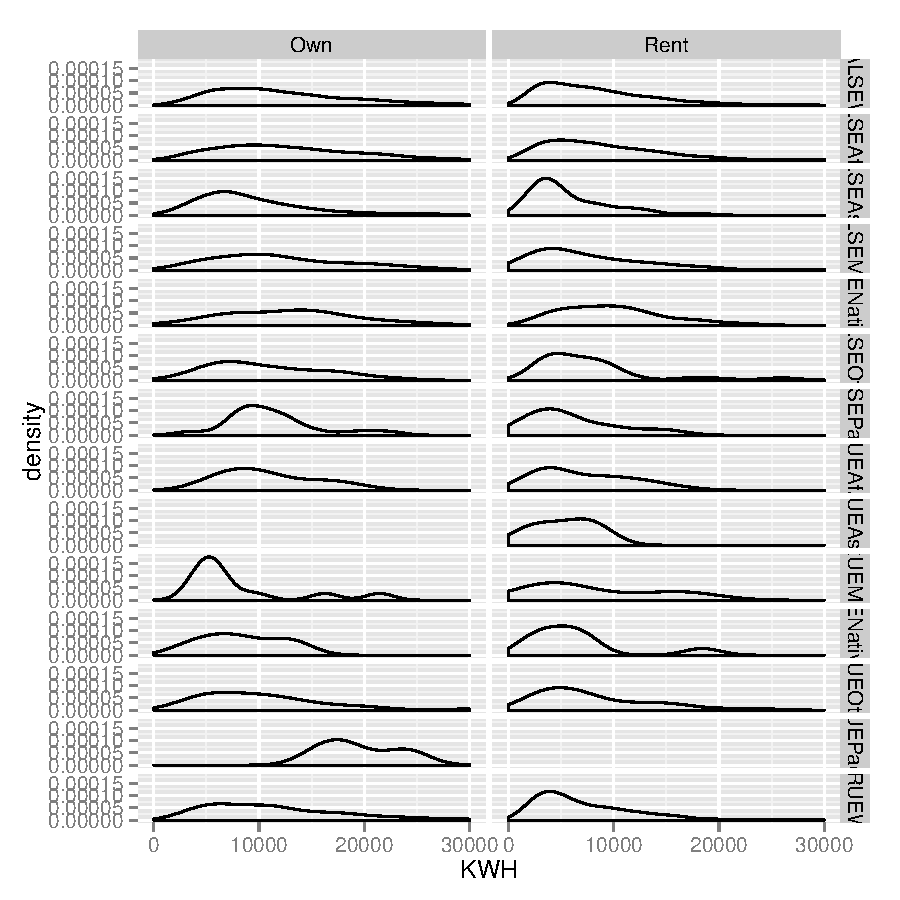
\includegraphics{DraftEdwardsWoods-005}
\end{center}
\end{figure}



\begin{figure}
\begin{center}
\caption{Annual kWh by Income}
\label{fig:kWhbyIncome}
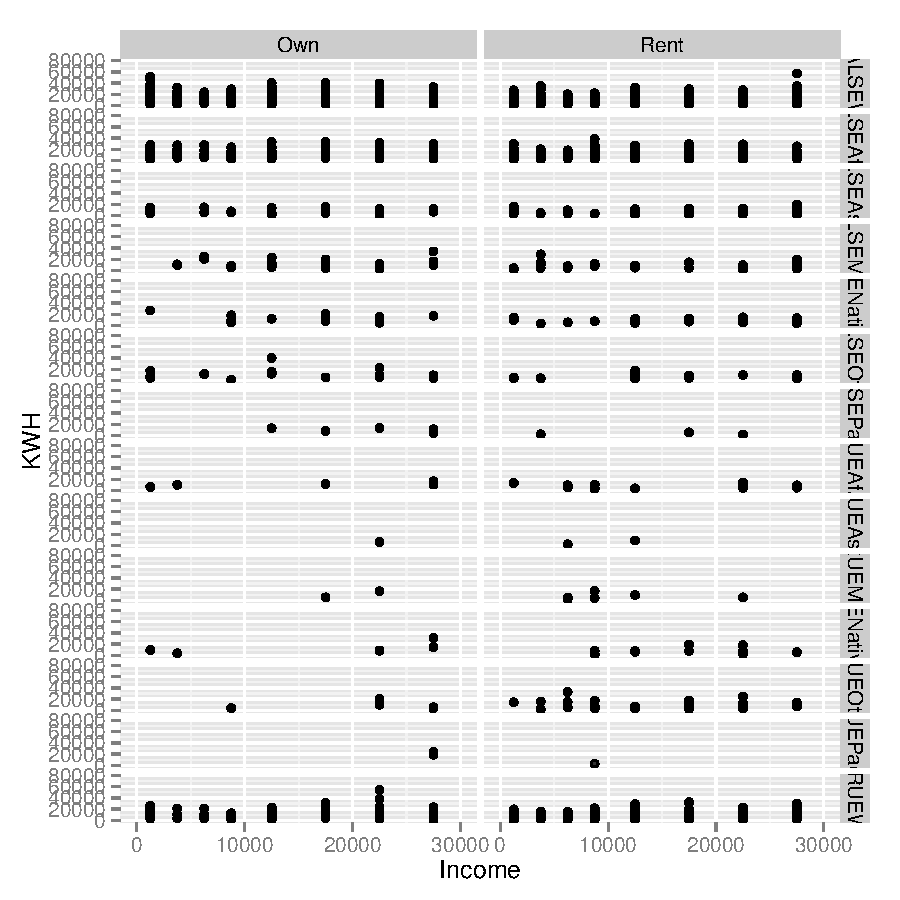
\includegraphics{DraftEdwardsWoods-006}
\end{center}
\end{figure}

\begin{figure}
\begin{center}\label{fig:HHbyRace}
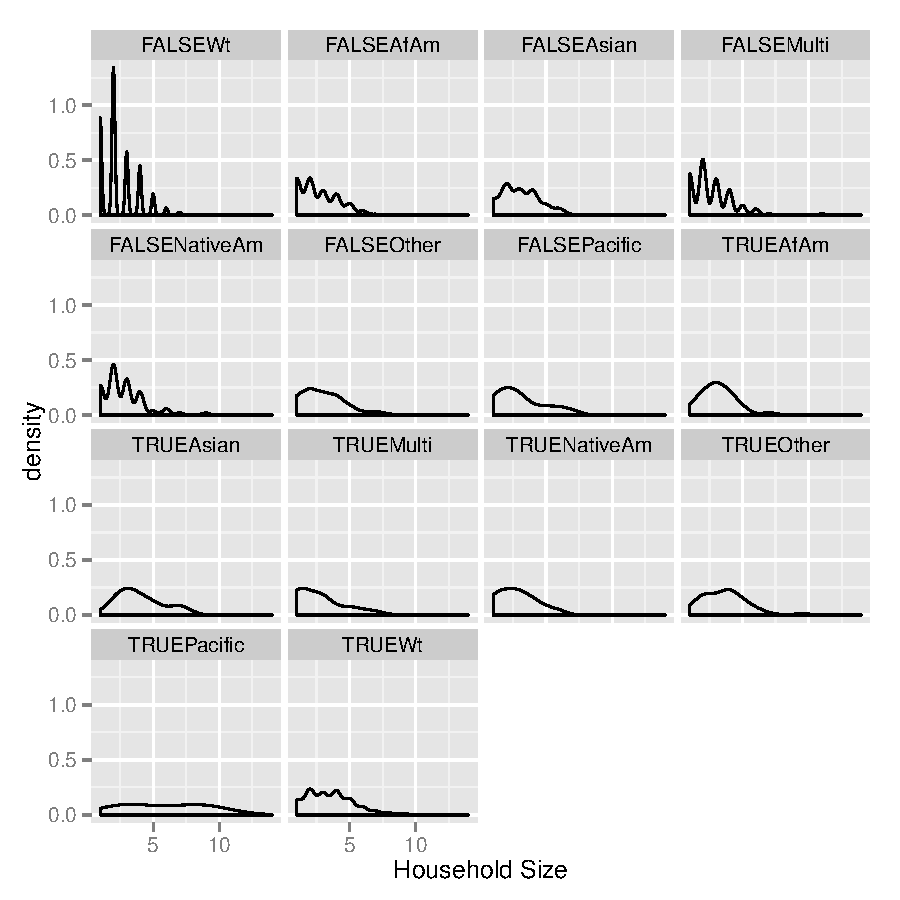
\includegraphics{DraftEdwardsWoods-007}
\end{center}
\end{figure}


  \subsection{Race and Ethnicity Differences in Equipment and Structure}

\begin{itemize}
  \item differences in structure type x
  \item difference in tenure x
  \item differences in energy star controlling for own rent
  \item general differences in own vs rent.  
  \item explain with split incentives story
  \item difference in age of structure x
  \item differences in hot water fuel x
  \item difference in heating fuel x
    \item difference in climate/location x
\end{itemize}
  
  


  
% latex table generated in R 3.1.3 by xtable 1.7-4 package
% Tue Mar 31 23:05:59 2015
\begin{table}[ht]
\centering
\begin{tabular}{rrr}
  \hline
 & FALSE & TRUE \\ 
  \hline
FALSEWt & 7606 & 384 \\ 
  FALSEAfAm & 1367 &  88 \\ 
  FALSEAsian & 424 &  21 \\ 
  FALSEMulti & 133 &  13 \\ 
  FALSENativeAm &  68 &   5 \\ 
  FALSEOther & 102 &   9 \\ 
  FALSEPacific &  30 &   6 \\ 
  TRUEAfAm &  31 &   3 \\ 
  TRUEAsian &   4 &   2 \\ 
  TRUEMulti &  19 &   2 \\ 
  TRUENativeAm &  36 &   1 \\ 
  TRUEOther &  88 &  11 \\ 
  TRUEPacific &   4 &   0 \\ 
  TRUEWt & 1330 & 118 \\ 
   \hline
\end{tabular}
\caption{EnergyStar Wall AC by Race and Ethnicity} 
\label{tab:EnergyStarWall}
\end{table}

% latex table generated in R 3.1.3 by xtable 1.7-4 package
% Tue Mar 31 23:05:59 2015
\begin{table}[ht]
\centering
\begin{tabular}{rrr}
  \hline
 & Rural & Urban \\ 
  \hline
FALSEWt & 1937 & 6053 \\ 
  FALSEAfAm & 192 & 1263 \\ 
  FALSEAsian &  14 & 431 \\ 
  FALSEMulti &  28 & 118 \\ 
  FALSENativeAm &  25 &  48 \\ 
  FALSEOther &  12 &  99 \\ 
  FALSEPacific &   4 &  32 \\ 
  TRUEAfAm &   6 &  28 \\ 
  TRUEAsian &   0 &   6 \\ 
  TRUEMulti &   1 &  20 \\ 
  TRUENativeAm &   3 &  34 \\ 
  TRUEOther &   5 &  94 \\ 
  TRUEPacific &   2 &   2 \\ 
  TRUEWt & 137 & 1311 \\ 
   \hline
\end{tabular}
\caption{Race by Urban/Rural} 
\label{tab:UrbRural}
\end{table}

% latex table generated in R 3.1.3 by xtable 1.7-4 package
% Tue Mar 31 23:05:59 2015
\begin{table}[ht]
\centering
\begin{tabular}{rrrrrrrrr}
  \hline
 & NG & LPG & Oil & Kerosene & Elec & Wood & Solar & Other \\ 
  \hline
FALSEWt & 4077 & 315 & 361 &   3 & 3190 &  11 &  12 &   7 \\ 
  FALSEAfAm & 755 &  17 &  35 &   0 & 640 &   0 &   2 &   0 \\ 
  FALSEAsian & 312 &   7 &  12 &   0 & 109 &   0 &   0 &   2 \\ 
  FALSEMulti &  85 &   5 &   3 &   0 &  53 &   0 &   0 &   0 \\ 
  FALSENativeAm &  34 &   2 &   1 &   0 &  36 &   0 &   0 &   0 \\ 
  FALSEOther &  57 &   3 &   6 &   0 &  44 &   0 &   0 &   0 \\ 
  FALSEPacific &  15 &   0 &   2 &   0 &  17 &   0 &   2 &   0 \\ 
  TRUEAfAm &  20 &   0 &   1 &   0 &  13 &   0 &   0 &   0 \\ 
  TRUEAsian &   5 &   0 &   0 &   0 &   1 &   0 &   0 &   0 \\ 
  TRUEMulti &  12 &   0 &   1 &   0 &   8 &   0 &   0 &   0 \\ 
  TRUENativeAm &  29 &   0 &   0 &   0 &   8 &   0 &   0 &   0 \\ 
  TRUEOther &  62 &   1 &   5 &   0 &  30 &   0 &   0 &   0 \\ 
  TRUEPacific &   1 &   1 &   0 &   0 &   2 &   0 &   0 &   0 \\ 
  TRUEWt & 830 &  33 &  26 &   0 & 552 &   0 &   1 &   0 \\ 
   \hline
\end{tabular}
\caption{Water Service by Race and Ethnicity} 
\label{tab:Water}
\end{table}
% latex table generated in R 3.1.3 by xtable 1.7-4 package
% Tue Mar 31 23:05:59 2015
\begin{table}[ht]
\centering
\begin{tabular}{rrrrrrrrrr}
  \hline
 & NG & LPG & Oil & Kerosene & Elec & Wood & Solar & District & Other \\ 
  \hline
FALSEWt & 3987 & 400 & 642 &  40 & 2515 & 245 &   1 &  11 &  19 \\ 
  FALSEAfAm & 674 &  29 &  60 &   6 & 640 &  10 &   0 &   5 &   0 \\ 
  FALSEAsian & 249 &   1 &  21 &   0 & 122 &   1 &   0 &   2 &   0 \\ 
  FALSEMulti &  80 &   6 &   7 &   0 &  41 &   7 &   0 &   0 &   1 \\ 
  FALSENativeAm &  34 &   3 &   1 &   0 &  33 &   2 &   0 &   0 &   0 \\ 
  FALSEOther &  59 &   1 &   9 &   0 &  36 &   3 &   0 &   0 &   0 \\ 
  FALSEPacific &  16 &   0 &   2 &   0 &   5 &   1 &   0 &   0 &   0 \\ 
  TRUEAfAm &  21 &   0 &   1 &   1 &   9 &   0 &   0 &   0 &   0 \\ 
  TRUEAsian &   4 &   0 &   0 &   0 &   1 &   0 &   0 &   0 &   0 \\ 
  TRUEMulti &  11 &   0 &   4 &   0 &   4 &   1 &   0 &   0 &   0 \\ 
  TRUENativeAm &  26 &   1 &   2 &   0 &   7 &   0 &   0 &   0 &   0 \\ 
  TRUEOther &  53 &   0 &   8 &   1 &  32 &   0 &   0 &   2 &   0 \\ 
  TRUEPacific &   1 &   0 &   0 &   0 &   2 &   0 &   0 &   0 &   0 \\ 
  TRUEWt & 604 &  25 &  51 &   2 & 540 &  18 &   0 &   3 &   1 \\ 
   \hline
\end{tabular}
\caption{Heating Fuel by Race and Ethnicity} 
\label{tab:HeatFuel}
\end{table}
% latex table generated in R 3.1.3 by xtable 1.7-4 package
% Tue Mar 31 23:05:59 2015
\begin{table}[ht]
\centering
\begin{tabular}{rrrrrr}
  \hline
 & VColdCold & HotDryMixedDry & HotHumid & MixedHumid & Marine \\ 
  \hline
FALSEWt & 3118 & 850 & 1216 & 2382 & 424 \\ 
  FALSEAfAm & 299 & 131 & 383 & 611 &  31 \\ 
  FALSEAsian &  95 & 128 &  60 &  77 &  85 \\ 
  FALSEMulti &  51 &  27 &  13 &  40 &  15 \\ 
  FALSENativeAm &  23 &  10 &   7 &  28 &   5 \\ 
  FALSEOther &  29 &  16 &  24 &  37 &   5 \\ 
  FALSEPacific &   4 &   6 &  13 &   4 &   9 \\ 
  TRUEAfAm &  16 &   5 &   4 &   9 &   0 \\ 
  TRUEAsian &   2 &   2 &   1 &   0 &   1 \\ 
  TRUEMulti &  12 &   6 &   1 &   0 &   2 \\ 
  TRUENativeAm &   9 &  14 &   1 &   8 &   5 \\ 
  TRUEOther &  35 &  19 &  10 &  28 &   7 \\ 
  TRUEPacific &   2 &   0 &   2 &   0 &   0 \\ 
  TRUEWt & 237 & 481 & 406 & 237 &  87 \\ 
   \hline
\end{tabular}
\caption{Climate by Race and Ethnicity} 
\label{tab:Climate}
\end{table}
\begin{figure}
\begin{center}
\caption{Age of Structure by Rent/Own and Race/Ethnicity}
\label{fig:AgebyOwnRace}
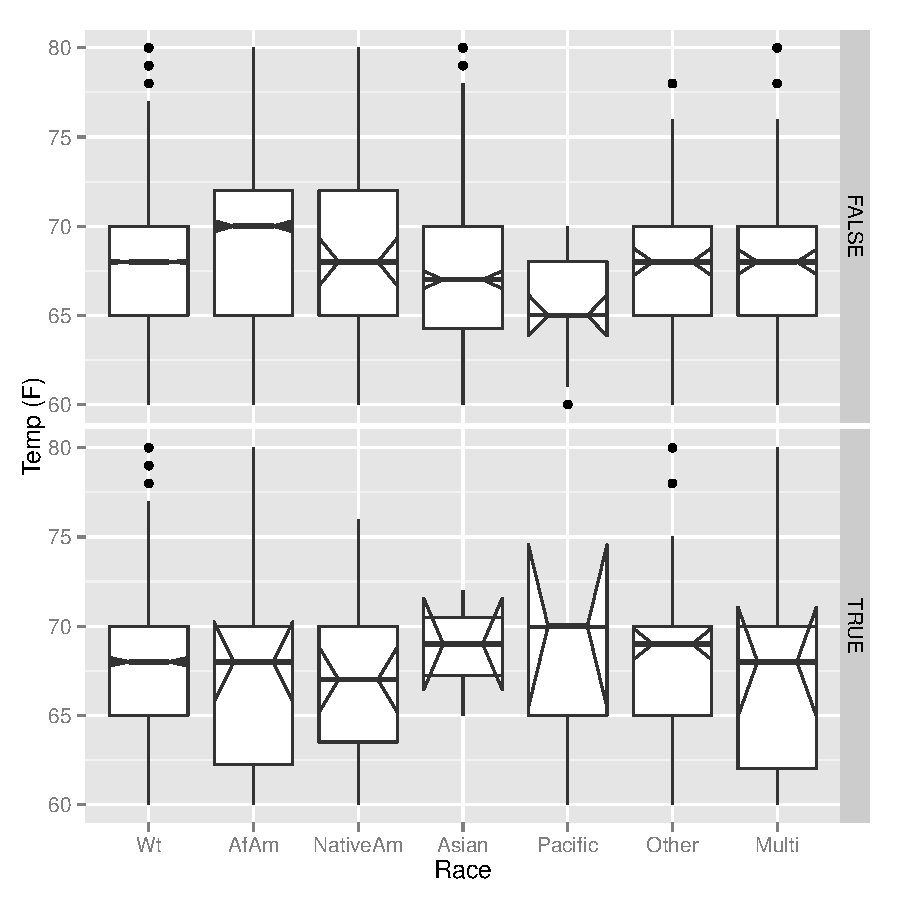
\includegraphics{DraftEdwardsWoods-013}
\end{center}
\end{figure}


\subsection{Differences in Reported Behavior}
  
  \begin{itemize}
    \item Differences in thermostat settings
    \item difference in cooking behavior x
    \item difference in reported AC use

  \end{itemize}
  
  
% latex table generated in R 3.1.3 by xtable 1.7-4 package
% Tue Mar 31 23:06:01 2015
\begin{table}[ht]
\centering
\begin{tabular}{rrrrrrrr}
  \hline
 & Never & ThreeDay & TwoDay & OneDay & FewWeek & OneWeek & LessWeek \\ 
  \hline
FALSEWt &  67 & 452 & 1814 & 3303 & 1825 & 254 & 275 \\ 
  FALSEAfAm &  11 & 156 & 351 & 341 & 448 &  80 &  68 \\ 
  FALSEAsian &   4 &  63 & 111 & 148 &  91 &  13 &  15 \\ 
  FALSEMulti &   2 &  14 &  45 &  40 &  36 &   7 &   2 \\ 
  FALSENativeAm &   0 &   7 &  22 &  27 &  11 &   3 &   3 \\ 
  FALSEOther &   2 &  10 &  25 &  21 &  43 &   3 &   7 \\ 
  FALSEPacific &   0 &   3 &   9 &  10 &  11 &   0 &   3 \\ 
  TRUEAfAm &   1 &   4 &   7 &  13 &   9 &   0 &   0 \\ 
  TRUEAsian &   0 &   0 &   1 &   3 &   2 &   0 &   0 \\ 
  TRUEMulti &   0 &   2 &   1 &  11 &   5 &   2 &   0 \\ 
  TRUENativeAm &   0 &   3 &  12 &  15 &   4 &   2 &   1 \\ 
  TRUEOther &   0 &  20 &  28 &  31 &  14 &   3 &   3 \\ 
  TRUEPacific &   0 &   3 &   0 &   1 &   0 &   0 &   0 \\ 
  TRUEWt &  22 & 208 & 453 & 435 & 226 &  42 &  62 \\ 
   \hline
\end{tabular}
\caption{Weekly Meals Cooked by Race and Ethnicity} 
\label{tab:Cooking}
\end{table}
\begin{figure}
\begin{center}
\caption{Daytime Temp and Race/Ethnicity (Winter)}
\label{fig:TempHomeRace}
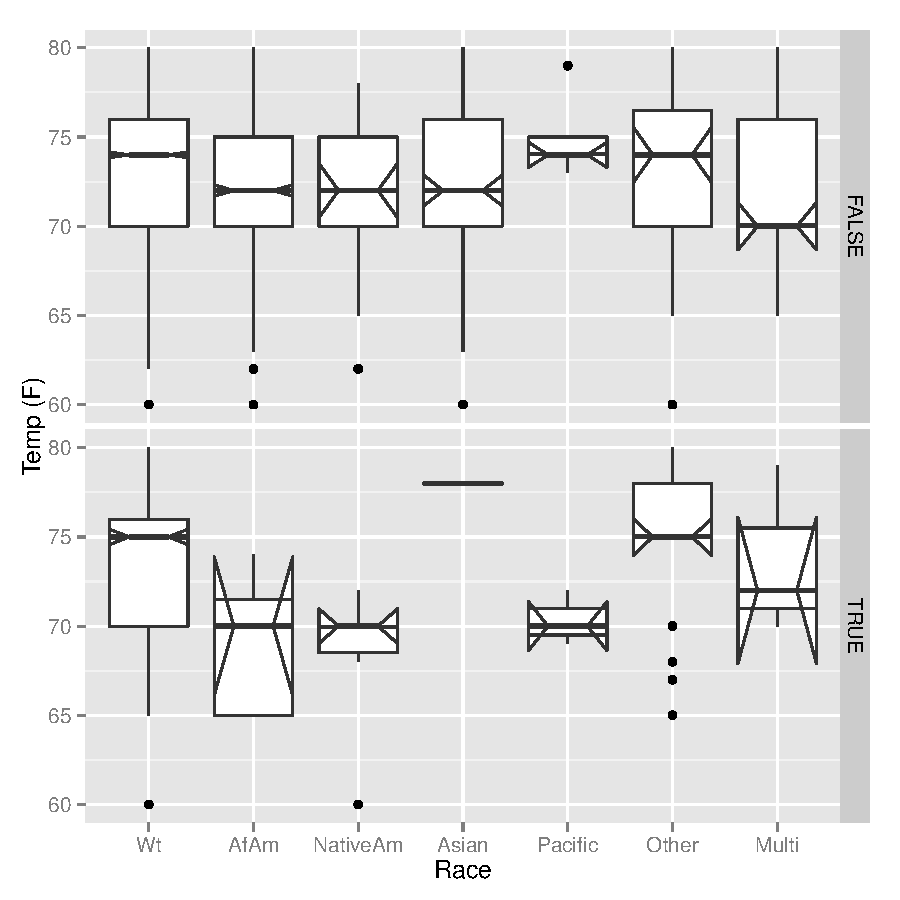
\includegraphics{DraftEdwardsWoods-015}
\end{center}
\end{figure}

\begin{figure}
\begin{center}
\caption{Daytime Temp When Away and Race/Ethnicity (Winter)}
\label{fig:DayAwayRace}
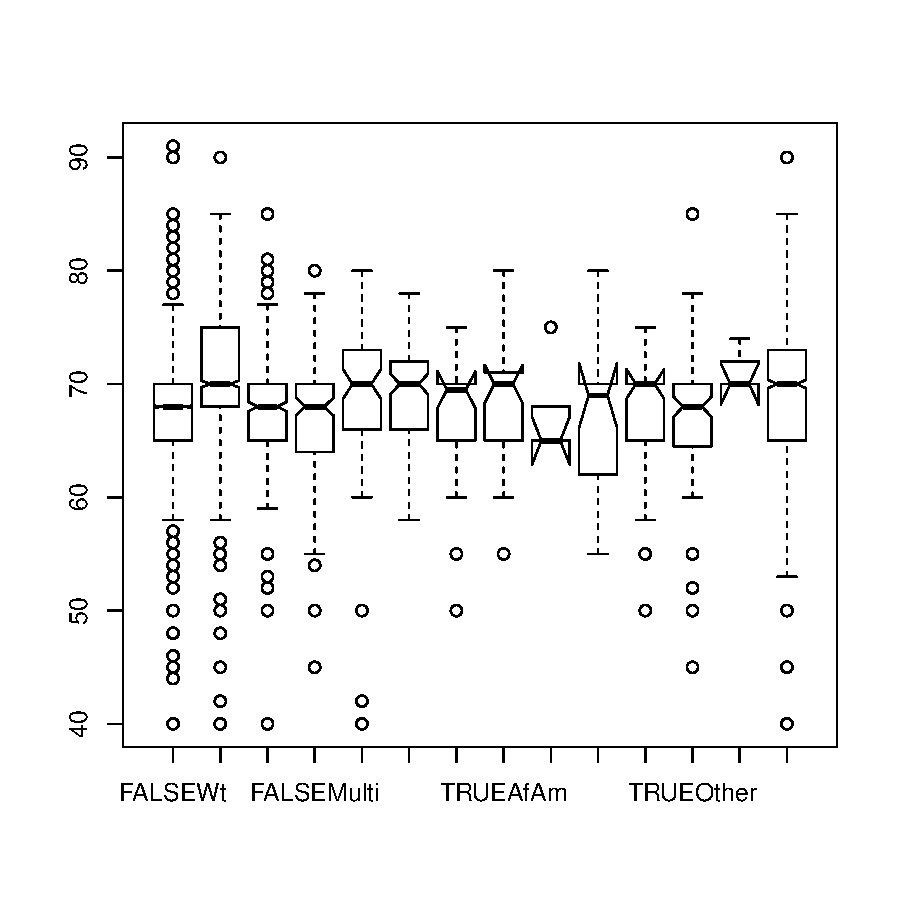
\includegraphics{DraftEdwardsWoods-016}
\end{center}
\end{figure}


\begin{figure}
\begin{center}
\caption{Nighttime Temp and Race/Ethnicity (Winter)}
\label{fig:NightRace}
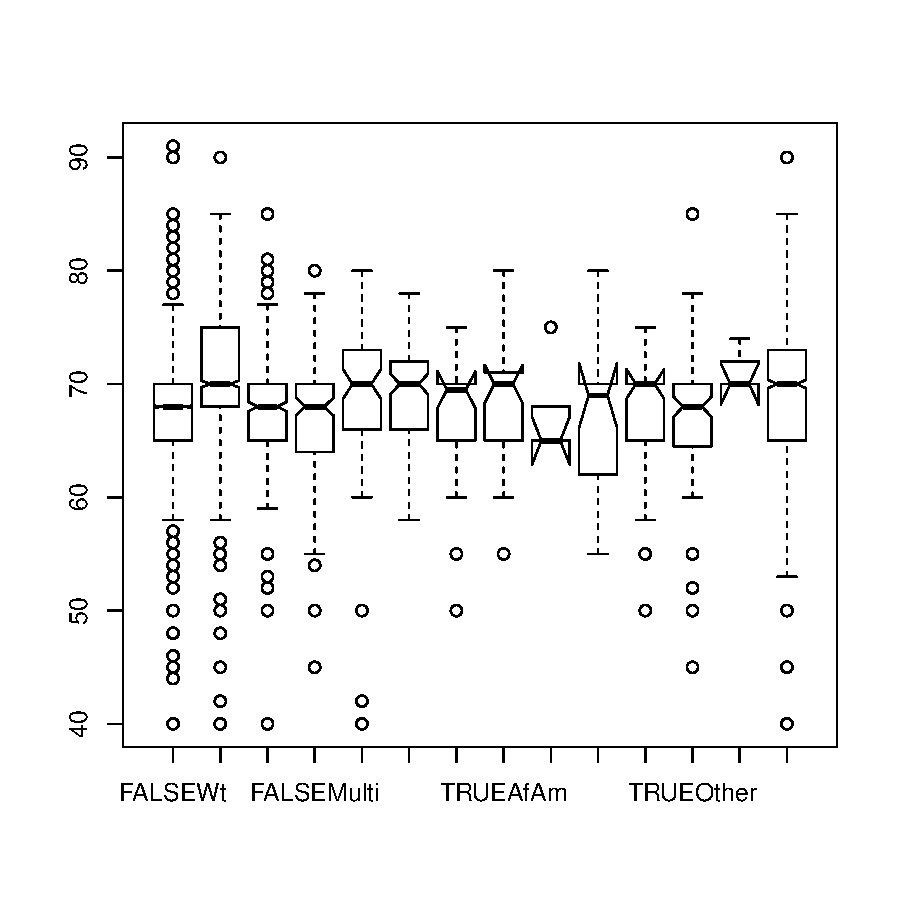
\includegraphics{DraftEdwardsWoods-017}
\end{center}
\end{figure}



\begin{figure}
\begin{center}
\caption{Daytime Temp Home by Race/Ethnicity (Summer)}
\label{fig:HomeRaceS}
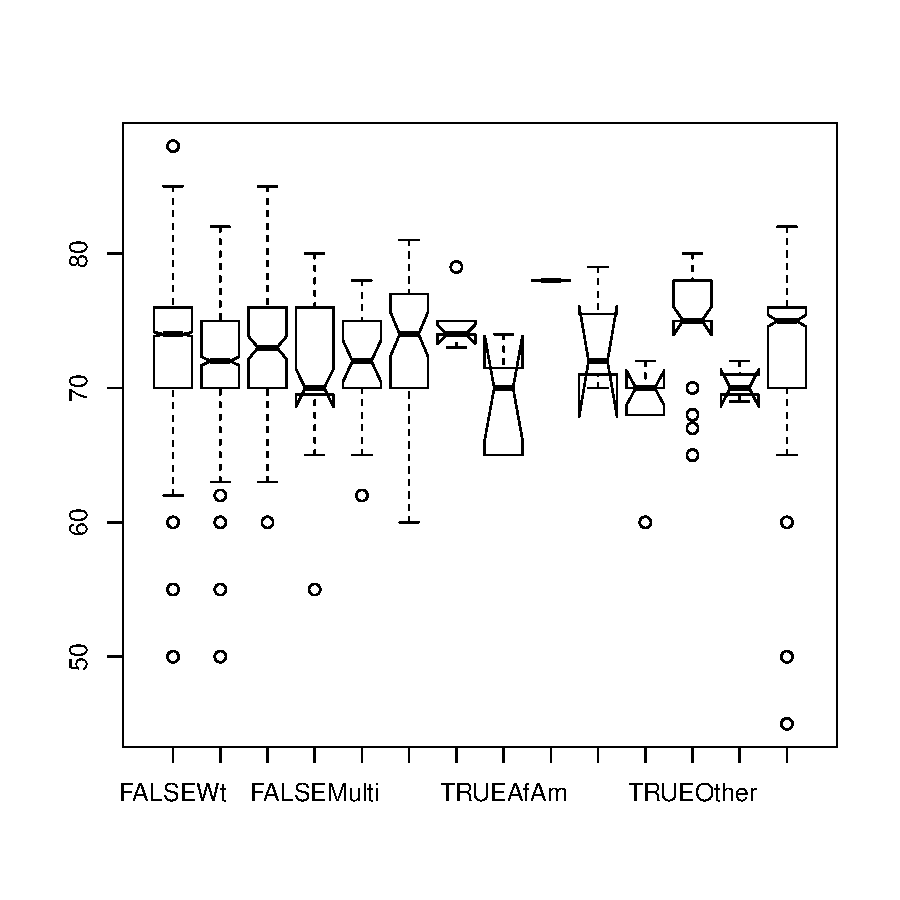
\includegraphics{DraftEdwardsWoods-018}
\end{center}
\end{figure}


\begin{figure}
\begin{center}
\caption{Day Temp Away by Race/Ethnicity (Summer)}
\label{fig:AwayRaceS}
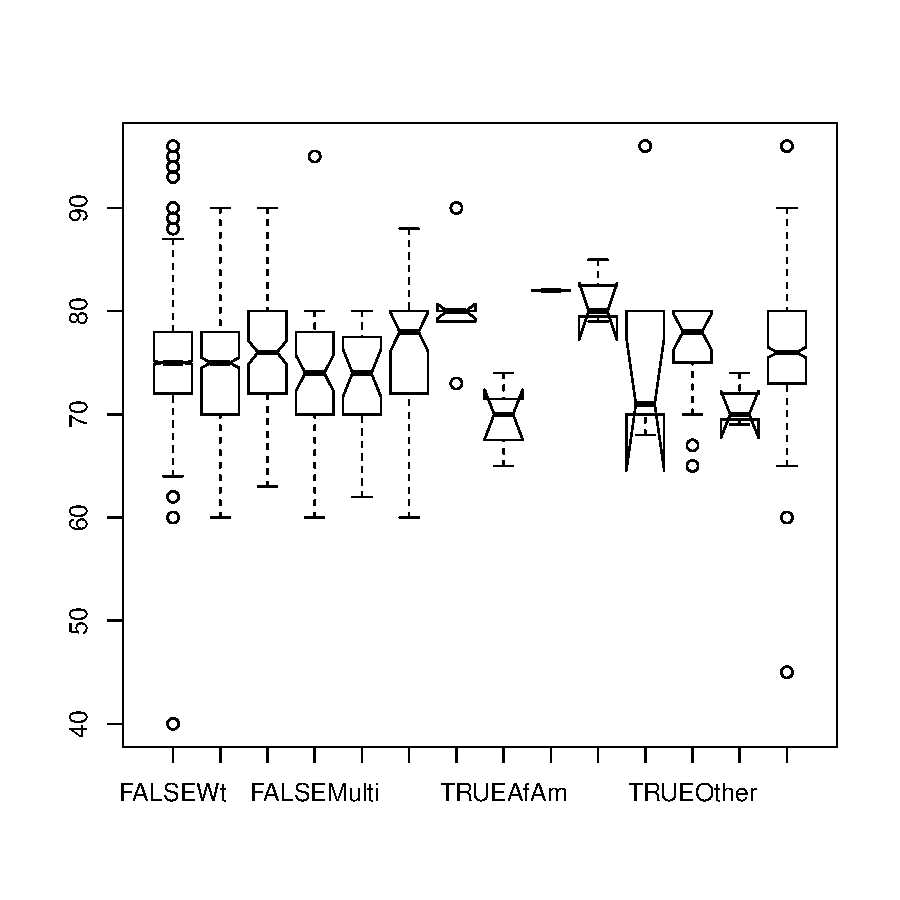
\includegraphics{DraftEdwardsWoods-019}
\end{center}
\end{figure}


\begin{figure}
\begin{center}
\caption{Nighttime Temp and Race/Ethnicity (Summer)}
\label{fig:NightRaceS}
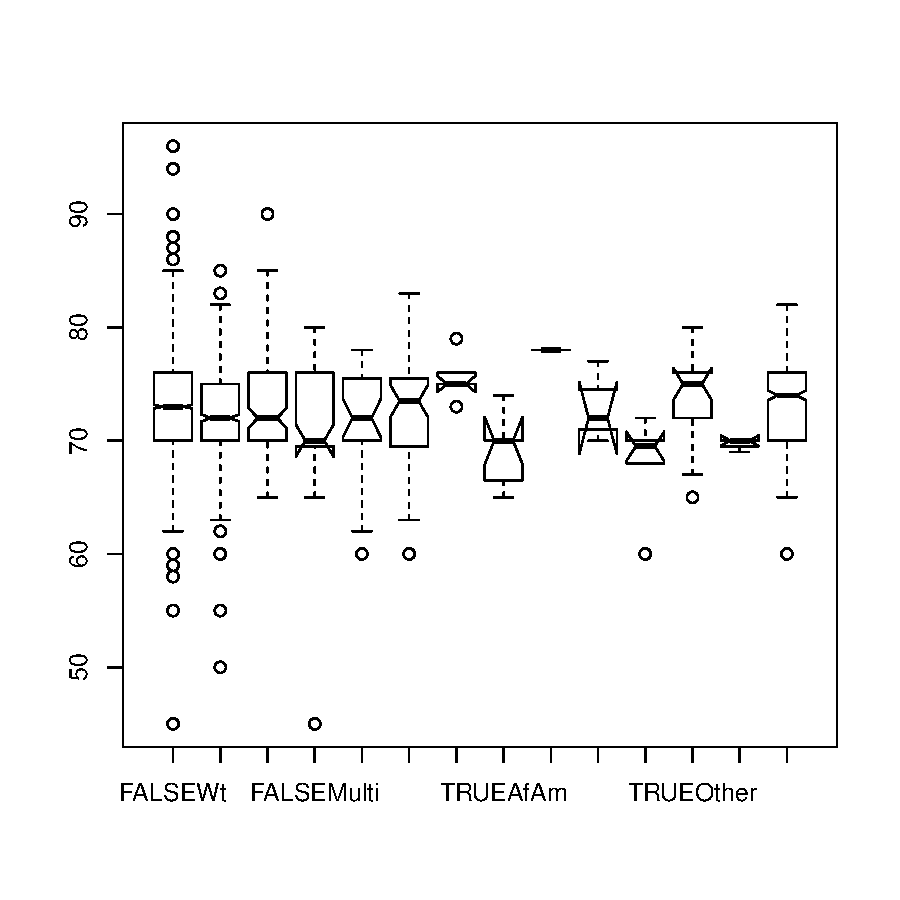
\includegraphics{DraftEdwardsWoods-020}
\end{center}
\end{figure}
  
  \subsection{HUD Complaints as a Measure of Discrimination}\label{sec:WhyHUD}
  
  \begin{itemize}
    \item trouble finding a good statewide index of housing discrimination
    \item the HUD complaint measure
    \item may be endogenous and be indicative of reduced discrimination
  
  \end{itemize}

% latex table generated in R 3.1.3 by xtable 1.7-4 package
% Tue Mar 31 23:06:01 2015
\begin{table}[ht]
\centering
\begin{tabular}{rllr}
  \hline
 & State & Population & Reports (per 100,000) \\ 
  \hline
1 & Alabama & 4,677,464 & 7.50 \\ 
  2 & Alaska & 688,125 & 13.01 \\ 
  3 & Arizona & 6,499,377 & 3.68 \\ 
  4 & Arkansas & 2,867,764 & 9.26 \\ 
  5 & California & 36,580,371 & 3.03 \\ 
  6 & Colorado & 4,935,213 & 1.97 \\ 
  7 & Connecticut & 3,502,932 & 20.50 \\ 
  8 & Delaware & 876,211 & 14.00 \\ 
  9 & District of Columbia & 590,074 & 14.00 \\ 
  10 & Florida & 18,423,878 & 3.93 \\ 
  11 & Georgia & 9,697,838 & 2.06 \\ 
  12 & Hawaii & 1,287,481 & 13.01 \\ 
  13 & Idaho & 1,527,506 & 9.94 \\ 
  14 & Illinois & 12,842,954 & 2.88 \\ 
  15 & Indiana & 6,388,309 & 9.14 \\ 
  16 & Iowa & 2,993,987 & 19.92 \\ 
  17 & Kansas & 2,797,375 & 10.31 \\ 
  18 & Kentucky & 4,287,931 & 7.50 \\ 
  19 & Louisiana & 4,451,513 & 9.26 \\ 
  20 & Maine & 1,319,691 & 20.50 \\ 
  21 & Maryland & 5,658,655 & 14.00 \\ 
  22 & Massachusetts & 6,543,595 & 4.51 \\ 
  23 & Michigan & 10,002,486 & 4.97 \\ 
  24 & Minnesota & 5,230,567 & 19.92 \\ 
  25 & Mississippi & 2,940,212 & 7.50 \\ 
  26 & Missouri & 5,956,335 & 4.99 \\ 
  27 & Montana & 968,035 & 9.94 \\ 
  28 & Nebraska & 1,781,949 & 10.31 \\ 
  29 & Nevada & 2,615,772 & 5.08 \\ 
  30 & New Hampshire & 1,321,872 & 20.50 \\ 
  31 & New Jersey & 8,663,398 & 2.34 \\ 
  32 & New Mexico & 1,986,763 & 5.08 \\ 
  33 & New York & 19,467,789 & 4.60 \\ 
  34 & North Carolina & 9,247,134 & 4.22 \\ 
  35 & North Dakota & 641,421 & 19.92 \\ 
  36 & Ohio & 11,528,072 & 9.14 \\ 
  37 & Oklahoma & 3,644,025 & 9.26 \\ 
  38 & Oregon & 3,782,991 & 13.01 \\ 
  39 & Pennsylvania & 12,566,368 & 1.87 \\ 
  40 & Rhode Island & 1,053,502 & 20.50 \\ 
  41 & South Carolina & 4,503,280 & 4.22 \\ 
  42 & South Dakota & 804,532 & 19.92 \\ 
  43 & Tennessee & 6,240,456 & 2.61 \\ 
  44 & Texas & 24,304,290 & 4.18 \\ 
  45 & Utah & 2,727,343 & 9.94 \\ 
  46 & Vermont & 621,049 & 20.50 \\ 
  47 & Virginia & 7,795,424 & 2.03 \\ 
  48 & Washington & 6,566,073 & 13.01 \\ 
  49 & West Virginia & 1,814,873 & 14.00 \\ 
  50 & Wisconsin & 5,627,610 & 1.81 \\ 
  51 & Wyoming & 532,981 & 9.94 \\ 
   \hline
\end{tabular}
\caption{HUD Complaints per 100,000 Population} 
\label{tab:HUDComplaints}
\end{table}
\section{Conditional Demand Estimation}

  \subsection{Orthodox Results}
  
  \begin{itemize}
    \item Emphasize that we are making better use of race and ethnicity as a control with income than is common.
    \item We are not using the same estimation method as in RECS estimates of end use.  Our model is much simpler and does not use engineering estimates or significant non-linearity.
    \item Major end-uses are included but relatively unsophisticated.
    \item discuss the orthodox results.
  \end{itemize}
  
  
  
Modern conditional demand models of the kind commonly created as part of the process of data collection of large residential appliance and use surveys such as RECS, include a mix of engineering estimates, survey responses and analyst best estimates to produce energy end-use estimates.  For example, survey respondents will give an age range on the furnace they have installed, the square footage of the residence, and some indication of heating set points.  The analyst will assign a likely efficiency for the furnace based on the average of the age ranges and then estimate hours used based on set points, weather, and the reported thermostat settings.  This produces estimates that are closer to a Statistically Adjusted Engineering (SAE) model than what is normally regarded as a conditional demand model outside of the energy community.

Our model is based more on the traditional conditional demand models, and includes terms for electricity use contingent on: the age of the home, which is a proxy for building code requirements and insulation; the weather, in the form of Heating and Cooling degree days with a base temperature of 65F; Meals cooked at home, to indicate energy use related to food preparation; the number and age of refrigerators, a major end-use;  the number of and types of TVs and computers, as a proxy for major plug loads; the existence of a well pump; weather the residence has electric hot water service; the existence of pools and hot tubs as well as if they are electrically heated; the kind of windows installed, as another indication of shell quality; the number of people in the home; and finally the income, race and ethnicity of the residents.  


Model: Multinomial logit
<<<<<<< HEAD
 old info  
=======

As a point of clarity, surveys with questions not filled in were coded with 97, to differentiate between responses that were left blank and those where the value coded was not applicable.  For the purpose of this paper 97s were recoded to not and were dropped from the analysis.  

>>>>>>> e6d97aa014adc48c0054c0608b702df1d6ec3cba
The multinomial logit is first ran with owndwel as the dependent variable and the independent variables as follows: income, educ, race5, age_1, age_2.  The base chosen was that of house renters, represented here as the first category (see appendix).  Here, race5 represents whether the head of the household is white.  Running the multinomial logit with all raises included as independent variables proved problematic, and largely insignificant.  Ages of children were left separate in an attempt to model the difference between households with children of all ages and those with only young children.  Having only young children may represent households in starter homes who are not necessarily well established.  As well households with children over the age of eighteen are essentially ignored and treated as adults.  Another iteration of the model is also down removing the children variables and instead using resident count.
The pseudo r-squared for the first model specified is 0.0912, which low it is important to bear in mind the problematic nature of interpreting pseudo r-squared values.  

Results:

The first and most likely indicator of home ownership within the structure type is income.  Here, we find in the results that the effect of income is statistically significant in each category accept the renting of townhomes.  Theory may suggest that, as mentioned earlier, row houses and townhomes in highly desirable neighborhoods especially historic neighborhoods are often rentals and as such might be rented by those with high incomes.  This question will remained unanswered within the scope of this study. 

 More importantly, the sign of the coefficient for income is positive for house ownership (approx. .22).  Continuing down the coefficients it is negative for townhouse rental (insignificant), positive for townhouse ownership, and the trend continues until that of mobile homes.  The income coefficient for mobile homes is negative for both rental and ownership, suggesting that a positive change in income has a negative effect on the probability of a household choosing a mobile home regardless if they are choosing to rent or buy.  It could be suggested that living in a mobile home is considered an inferior good, and households might choose to forego ownership or renting a mobile home in favor of choosing any other domicile.
 
The education variable is estimated, and is found to be statistically insignificant in the ownership of houses and the renting of townhouses and small complex apartment units.  Based on its coefficient, its value as an explanatory variable appears to be weak, yet as we go down the list of owndwel values the education coefficient moves from a positive to a negative at mobile homes. That is to say that here, education appears to have an effect mostly positive between the owndwel values of 3-8, and negative thereafter.

Race, the dummy for being white, is statistically significant everywhere except in the rental of apartments in large small complexes.  Note that for mobile homes the dummy for race takes on a value of approximately 1 and 1.57 for renters and owners respectively.  This would suggest, while not realistic probabilities, that overwhelmingly whites have a higher probability of choosing mobile homes in comparison to non-self-reporting whites.  Notably, no results of interest were found regarding the stereotype of Native-Americans dwelling in mobile homes within the data.  Also race in this case appears to be linked to ownership of homes in each of the categories, within the bootstrapped version of the model it is statistically significant in each of the ownership owndwel categories.  

Age of children was found to be statistically significant in both variables largely.  The exceptions to the significance are in age_1, children under five for both large and small apartment complexes where households rent as well as the rental of mobile homes.  It is important to note that in each category the value of age_1 and age_2 coefficients is negative, which adds very little to our interpretations of the model.  Further, when we replace the children variables with that of resident count in the model we obtain a similar result where all coefficients are negative, and all statistically significant, in comparison to our base of house rental. 

When the model as specified first, is ran using a multinomial logit vce bootstrapping the results are slightly different with regards to children.  Now, while in places not statistically significant (see appendix) there does appear to be a trend towards the results are the same.  Further examination is needed.

%Fix latex ref
The parameter estimates of the full model can be found in appendix 
% \ref{OrthResults}
, partial results are shown in table 
% \ref{tab:ParOrthKWH}
.
  
% latex table generated in R 3.1.3 by xtable 1.7-4 package
% Tue Mar 31 23:06:02 2015
\begin{longtable}{rrrrr}
  \hline
 & Estimate & Std. Error & t value & Pr($>$$|$t$|$) \\ 
  \hline
Income & 0.0086 & 0.0016 & 5.3662 & 0.0000 \\ 
  Income:EthRaceFALSEAfAm & 0.0031 & 0.0027 & 1.1389 & 0.2548 \\ 
  Income:EthRaceFALSEAsian & -0.0243 & 0.0034 & -7.1646 & 0.0000 \\ 
  Income:EthRaceFALSEMulti & -0.0168 & 0.0069 & -2.4259 & 0.0153 \\ 
  Income:EthRaceFALSENativeAm & 0.0117 & 0.0123 & 0.9493 & 0.3425 \\ 
  Income:EthRaceFALSEOther & -0.0249 & 0.0083 & -2.9909 & 0.0028 \\ 
  Income:EthRaceFALSEPacific & -0.0163 & 0.0138 & -1.1807 & 0.2378 \\ 
  Income:EthRaceTRUEAfAm & -0.0120 & 0.0165 & -0.7271 & 0.4672 \\ 
  Income:EthRaceTRUEAsian & -0.0365 & 0.0454 & -0.8032 & 0.4219 \\ 
  Income:EthRaceTRUEMulti & -0.0291 & 0.0212 & -1.3745 & 0.1693 \\ 
  Income:EthRaceTRUENativeAm & -0.0187 & 0.0148 & -1.2599 & 0.2077 \\ 
  Income:EthRaceTRUEOther & -0.0262 & 0.0099 & -2.6335 & 0.0085 \\ 
  Income:EthRaceTRUEPacific & -0.0122 & 0.0380 & -0.3221 & 0.7474 \\ 
  Income:EthRaceTRUEWt & -0.0192 & 0.0031 & -6.2907 & 0.0000 \\ 
  StrTenureOwnSFDetached:TOTSQFT\_EN:HDD65 & 0.0001 & 0.0000 & 4.1043 & 0.0000 \\ 
  StrTenureOwnLgApartment:TOTSQFT\_EN:HDD65 & -0.0001 & 0.0001 & -0.9580 & 0.3381 \\ 
  StrTenureOwnMobile:TOTSQFT\_EN:HDD65 & 0.0004 & 0.0001 & 5.9838 & 0.0000 \\ 
  StrTenureOwnSFAttached:TOTSQFT\_EN:HDD65 & -0.0000 & 0.0000 & -0.5516 & 0.5812 \\ 
  StrTenureOwnSmApartment:TOTSQFT\_EN:HDD65 & 0.0000 & 0.0001 & 0.5438 & 0.5866 \\ 
  StrTenureRentLgApartment:TOTSQFT\_EN:HDD65 & -0.0002 & 0.0001 & -4.0031 & 0.0001 \\ 
  StrTenureRentMobile:TOTSQFT\_EN:HDD65 & 0.0004 & 0.0002 & 1.7633 & 0.0779 \\ 
  StrTenureRentSFAttached:TOTSQFT\_EN:HDD65 & 0.0000 & 0.0001 & 0.6010 & 0.5479 \\ 
  StrTenureRentSFDetached:TOTSQFT\_EN:HDD65 & 0.0000 & 0.0000 & 0.5515 & 0.5813 \\ 
  StrTenureRentSmApartment:TOTSQFT\_EN:HDD65 & -0.0001 & 0.0001 & -1.8580 & 0.0632 \\ 
  StrTenureOwnSFDetached:TOTSQFT\_EN:CDD65 & 0.0008 & 0.0000 & 19.2068 & 0.0000 \\ 
  StrTenureOwnLgApartment:TOTSQFT\_EN:CDD65 & -0.0002 & 0.0002 & -0.8168 & 0.4140 \\ 
  StrTenureOwnMobile:TOTSQFT\_EN:CDD65 & 0.0009 & 0.0001 & 7.3167 & 0.0000 \\ 
  StrTenureOwnSFAttached:TOTSQFT\_EN:CDD65 & 0.0006 & 0.0001 & 5.0127 & 0.0000 \\ 
  StrTenureOwnSmApartment:TOTSQFT\_EN:CDD65 & 0.0001 & 0.0003 & 0.4022 & 0.6875 \\ 
  StrTenureRentLgApartment:TOTSQFT\_EN:CDD65 & 0.0000 & 0.0001 & 0.3926 & 0.6946 \\ 
  StrTenureRentMobile:TOTSQFT\_EN:CDD65 & 0.0024 & 0.0004 & 6.3205 & 0.0000 \\ 
  StrTenureRentSFAttached:TOTSQFT\_EN:CDD65 & 0.0007 & 0.0002 & 4.0210 & 0.0001 \\ 
  StrTenureRentSFDetached:TOTSQFT\_EN:CDD65 & 0.0008 & 0.0001 & 9.2680 & 0.0000 \\ 
  StrTenureRentSmApartment:TOTSQFT\_EN:CDD65 & 0.0005 & 0.0002 & 2.8365 & 0.0046 \\ 
   \hline
\hline
\caption{Orthodox kWh Model} 
\label{tab:OrthoKWHLimited}
\end{longtable}
The top parameter, Income, shows the estimate for annual kWh per dollar of income for a household headed by a non-Hispanic Caucasian.  The remaining income related variables show the deviations from this case for Hispanic headed households, labeled TRUE in the table, and by the other self reported races.  Note that in all cases, with the exception of non-Hispanic Native Americans, the parameter estimates show less electricity used than non-Hispanic Caucasian households.  Only a few of these differences are statistically significant, non-Hispanic Asian and multi-ethnic households, as well as Hispanic Caucasian households and households that reported some other race.

The remaining items shown in the table show the electricity use per square foot for each of the structure types, e.g., Single Family Detached, and tenure, i.e., Rent or Own, per annual heating and cooling degree days.  Aside from the negative and significant estimate for the heating load in large Rented apartments, the results are unremarkable. 

\subsection{Endogenizing Structure and Other Variables}\label{sec:SingleEq}

Treating structure type and square footage as endogenous is our first step in estimating conditional demand for many end uses treating the choice of things like, EnergyStar appliances, refrigerator size and design.  The current standard, treating these as exogenous drivers of energy use biases or estimates of energy use in unknown ways.

Focusing on tenure, i.e., the decision to own or rent, structure and square footage decisions allows us to see if other housing market institutions are driving energy use differently depending on ethnicity.  At this early stage of research we are focusing only on these major drivers but we can expand the analysis to other choices including clothes washing, hot water service and other large energy drivers.

As stated in section \ref{sec:WhyHUD}, using HUD complaints as a measure of housing market discrimination based on race and ethnicity is less than optimal measure, but at this early stage is an adequate measure to determine the scale of the effect.  


Table 
% \ref{tab:OrthoSQFTLimited} 
shows only the discrimination related results for our model of square footage.  Full results can be seen in appendix 
% \ref{OrthResults}
.   Note that the square footage model includes structure type and tenure as an exogenous variable.  This model of square footage will be included later as part of a system estimation of electricity use.   

The key discrimination variable, reporttot, is the count of complaints received by HUD per 100,000 people in the state where the household is located. We interacted this variable with race and ethnicity to allow for different effects  groups but we do not allow the discrimination to vary by state. Note that the effects of HUD reports on square footage are rarely significant, only strongly significant for Hispanic Caucasian households.  In this case incidences of HUD complaints per 100,000 of state population results in a reduction in the square footage for Caucasian Hispanics by 22.73 square feet.


% \begin{itemize}
%   \item explain the logic behind the making both sqft and structure tenure endogenous.
%   \item primarily that sqft may be related to quality of houseing, newer structures
% \end{itemize}



While the impact of housing market discrimination has some effect on the size of residences, the effects on the ownership and structure type decision is expected to be more dramatic.  Housing market discrimination can be expected to push some people away from owned property and into the rental market, which is rife with split incentives for conservation and energy efficiency investments.  

Discrimination can also be a force pushing some households into structure types, where even when owned, that have significant split incentives for energy efficiency investments.  Take, for example, small and large apartment buildings.  While the householder may have control over some appliances, the building shell and some of the heating and cooling equipment decisions are made by others.  

Our model of structure type and tenure includes categories for both owned and rented: Large Apartments, Small Apartments, Mobile Homes, Single Family Detached, and Single Family Attached.  We explain the joint tenure and structure type with: the square footage of the structure, if the household receives rental assistance, Income, number of people in the household, education level of the head of household, the HUD reports per 100,000 in that state and whether the household is in a rural or urban location.  As in the square footage model, HUD reports are interacted with the race and ethnicity variables to allow for separate discrimination effects for each.


All parameter estimates for the models are statistically significant at the 1\% level and are displayed in appendix 
% \ref{OrthResults}. 


%Fix the Latex part of this.
Since all the parameters are statistically significant it is easier to show the effects of our measure of housing market discrimination on the probability of each structure and tenure choice for the race and ethnicity combinations.  The HUD reports run from 1.81249 complaints per 100,000 to 20.496 complaints per 100,000.  Figure 
% \ref{fig:HUDOnChoice} 
shows the reaction to HUD complaints over the 1 to 21 complaint range.


% 
% \begin{figure}
% \begin{center}\label{fig:HUDOnChoice}
% 
% <<echo=false,fig=TRUE>>=
% # Need to figure this figure out.  It may be very complex
% 
% @
% \end{center}
% \end{figure}

***Lots of explanation goes here***




  \subsection{System Estimation}

The single equation results discussed in section \ref{sec:SingleEq} show strong promise for endogenizing some of the decisions made about structure and equipment within the conditional demand model as well as the potential importance of housing market discrimination in structure choice.  In this section we treat square footage, tenure and structure type as endogenous and estimate estimate the electricity, structure/tenure, and square footage model as a system.

It is unclear how this can be accomplished in a full information, so we chose a two-state least squares technique estimating first the square footage model, then using forecasted values to estimate tenure and structure type model.  Forecasts from that model were used to resestimate and produce a new round of forecasts for the square footage model.  Both the forecasts of the structure tenure model and square footage model were then used to estimate the conditional demand model.

This should produce consistent results but the variance of the parameter estimates are biased.  It is unclear how to make the usual corrections to the variance of the parameter estimates given that the structure and tenure model is estimated as a multinomial logit.  The best alternative is to bootstrap the system.  There are a few caveats.

First, the bootstrap sampling is stratified so that all parameter estimates in all models can be estimated.  This is particularly important in the structure and tenure model.  We had to ensure enough observations of the rare endogenouse cells, rented mobile homes being the most restricted, and exogenous variables, e.g., Hispanic Pacific Islanders.  This was accomplished by simple rejection sampling rather than assigning different probabilities of selection to each of the cells.

Second, we did not censor non-positive square footage forecasts.  The square footage model is weaker than expected and it was quite possible to have negative forecasts.  Alternative models, such as Tobit, would not be effective, but we are considering transformations of square footage as we move forward.  

Finally, only 400 bootstrap replicates were evaluated.  This is usually enough to produce adequate estimates of the standard deviations of the parameter estimates in the electricity model but insufficient for BCa, percentile, or even basic bootstrap confidence intervals. 

% \begin{itemize}
%   \item results are bootstrapped 400 times for standard deviation estimates.  More can be done.
%   \item probablities of structure type rather than forecast were used.
%   \item no censoring for square footage less than zero.
%   \item boot strap samples were restricted to samples that allowed for all parameters to be estimated.
% \end{itemize}




% latex table generated in R 3.1.3 by xtable 1.7-4 package
% Tue Mar 31 23:06:03 2015
\begin{longtable}{rrrrl}
  \hline
 & Estimate & Std. Error & t value & Sig \\ 
  \hline
(Intercept) & -637.3566 & 1754.7664 & -0.3632 &   \\ 
  ElecMealsThreeDay & 1265.5101 & 447.0979 & 2.8305 & * \\ 
  ElecMealsTwoDay & 1548.2300 & 199.6619 & 7.7543 & *** \\ 
  ElecMealsOneDay & 1607.3686 & 186.4168 & 8.6224 & *** \\ 
  ElecMealsFewWeek & 1371.7940 & 201.0134 & 6.8244 & *** \\ 
  ElecMealsOneWeek & 1613.9994 & 446.8554 & 3.6119 & ** \\ 
  ElecMealsLessWeek & 1078.7643 & 420.7528 & 2.5639 & . \\ 
  NUMFRIG & 2043.1588 & 162.1146 & 12.6032 & *** \\ 
  AgeFridge2to4Years & -37.2321 & 219.9343 & -0.1693 &   \\ 
  AgeFridge5to9Years & 189.4846 & 206.9121 & 0.9158 &   \\ 
  AgeFridge20PlusYears & 289.0881 & 442.9034 & 0.6527 &   \\ 
  AgeFridge10to14Years & 390.5240 & 258.1351 & 1.5129 &   \\ 
  AgeFridge15to19Years & -109.7635 & 303.2599 & -0.3619 &   \\ 
  NUMPC & 431.9238 & 75.4693 & 5.7232 & *** \\ 
  TIMEON1OneTo3Hrs & 9.2777 & 182.6120 & 0.0508 &   \\ 
  TIMEON1ThreeTo6Hrs & 35.3052 & 208.4801 & 0.1693 &   \\ 
  TIMEON1SixTo10Hrs & 258.4370 & 294.7298 & 0.8769 &   \\ 
  TIMEON1Gr10 & 929.5422 & 268.3058 & 3.4645 & ** \\ 
  WELLPUMPTRUE & 1182.7020 & 300.5331 & 3.9353 & ** \\ 
  ElecWaterSmall & 4283.1501 & 307.1885 & 13.9431 & *** \\ 
  ElecWaterMed & 4381.2889 & 201.2909 & 21.7660 & *** \\ 
  ElecWaterLrg & 5695.3238 & 300.4903 & 18.9534 & *** \\ 
  ElecWaterTankless & 3171.8175 & 981.4629 & 3.2317 & * \\ 
  SWIMPOOLTRUE & 3603.9817 & 373.1464 & 9.6584 & *** \\ 
  ElecPoolTRUE & 5374.6889 & 1639.6680 & 3.2779 & * \\ 
  RECBATHTRUE & 1865.3790 & 679.7961 & 2.7440 & * \\ 
  ElecTubTRUE & 285.6194 & 837.6762 & 0.3410 &   \\ 
  NHSLDMEM & 729.8552 & 122.3334 & 5.9661 & *** \\ 
  Income & -0.0041 & 0.0051 & -0.8119 &   \\ 
  TVONWD1LessHour:TVTYPE1Standard & -2947.9784 & 1670.0620 & -1.7652 &   \\ 
  TVONWD1OneTo3Hrs:TVTYPE1Standard & -2737.2962 & 1647.3265 & -1.6617 &   \\ 
  TVONWD1ThreeTo6Hrs:TVTYPE1Standard & -2247.1394 & 1644.9601 & -1.3661 &   \\ 
  TVONWD1SixTo10Hrs:TVTYPE1Standard & -1636.5569 & 1631.4463 & -1.0031 &   \\ 
  TVONWD1Gr10:TVTYPE1Standard & -1264.7108 & 1695.0911 & -0.7461 &   \\ 
  TVONWD1LessHour:TVTYPE1LCD & -2621.5762 & 1669.7693 & -1.5700 &   \\ 
  TVONWD1OneTo3Hrs:TVTYPE1LCD & -1954.0084 & 1665.3302 & -1.1733 &   \\ 
  TVONWD1ThreeTo6Hrs:TVTYPE1LCD & -1610.0720 & 1655.8743 & -0.9723 &   \\ 
  TVONWD1SixTo10Hrs:TVTYPE1LCD & -1408.2089 & 1669.2281 & -0.8436 &   \\ 
  TVONWD1Gr10:TVTYPE1LCD & -203.9791 & 1659.1510 & -0.1229 &   \\ 
  TVONWD1LessHour:TVTYPE1Plasma & -676.0979 & 2140.4093 & -0.3159 &   \\ 
  TVONWD1OneTo3Hrs:TVTYPE1Plasma & -1233.2818 & 1733.7213 & -0.7113 &   \\ 
  TVONWD1ThreeTo6Hrs:TVTYPE1Plasma & -1844.3686 & 1686.0443 & -1.0939 &   \\ 
  TVONWD1SixTo10Hrs:TVTYPE1Plasma & -879.7077 & 1721.9584 & -0.5109 &   \\ 
  TVONWD1Gr10:TVTYPE1Plasma & 554.6818 & 1802.5056 & 0.3077 &   \\ 
  TVONWD1LessHour:TVTYPE1Projection & -904.5303 & 1882.4580 & -0.4805 &   \\ 
  TVONWD1OneTo3Hrs:TVTYPE1Projection & -1684.0750 & 1658.0657 & -1.0157 &   \\ 
  TVONWD1ThreeTo6Hrs:TVTYPE1Projection & -1765.5157 & 1690.0189 & -1.0447 &   \\ 
  TVONWD1SixTo10Hrs:TVTYPE1Projection & -439.8397 & 1733.8849 & -0.2537 &   \\ 
  TVONWD1Gr10:TVTYPE1Projection & 1590.1129 & 1862.2353 & 0.8539 &   \\ 
  TVONWD1LessHour:TVTYPE1LED & -5170.4567 & 2364.0640 & -2.1871 &   \\ 
  TVONWD1OneTo3Hrs:TVTYPE1LED & -1215.2448 & 1872.4922 & -0.6490 &   \\ 
  TVONWD1ThreeTo6Hrs:TVTYPE1LED & -1562.8906 & 1770.5880 & -0.8827 &   \\ 
  TVONWD1SixTo10Hrs:TVTYPE1LED & -3383.2738 & 2128.9419 & -1.5892 &   \\ 
  TVONWD1Gr10:TVTYPE1LED &  &  &  &  \\ 
  PSQFT:TYPEGLASSSinglePane & 1.1013 & 0.3369 & 3.2685 & * \\ 
  PSQFT:TYPEGLASSDoublePane & 1.2790 & 0.3266 & 3.9161 & ** \\ 
  PSQFT:TYPEGLASSTriplePane & 1.6324 & 0.3966 & 4.1163 & *** \\ 
  Income:EthRaceFALSEAfAm & -0.0015 & 0.0038 & -0.3974 &   \\ 
  Income:EthRaceFALSEAsian & -0.0218 & 0.0047 & -4.5984 & *** \\ 
  Income:EthRaceFALSEMulti & -0.0143 & 0.0071 & -2.0102 &   \\ 
  Income:EthRaceFALSENativeAm & 0.0075 & 0.0244 & 0.3065 &   \\ 
  Income:EthRaceFALSEOther & -0.0180 & 0.0088 & -2.0539 &   \\ 
  Income:EthRaceFALSEPacific & -0.0160 & 0.0244 & -0.6564 &   \\ 
  Income:EthRaceTRUEAfAm & -0.0096 & 0.0158 & -0.6088 &   \\ 
  Income:EthRaceTRUEAsian & -0.0339 & 0.0446 & -0.7606 &   \\ 
  Income:EthRaceTRUEMulti & -0.0376 & 0.0224 & -1.6760 &   \\ 
  Income:EthRaceTRUENativeAm & -0.0133 & 0.0123 & -1.0784 &   \\ 
  Income:EthRaceTRUEOther & -0.0338 & 0.0094 & -3.5969 & ** \\ 
  Income:EthRaceTRUEPacific & 0.0266 & 0.4360 & 0.0609 &   \\ 
  Income:EthRaceTRUEWt & -0.0211 & 0.0045 & -4.6937 & *** \\ 
  PSQFT:OwnSFDetached:HDD65 & 0.0001 & 0.0000 & 4.1986 & *** \\ 
  PSQFT:HDD65:OwnLgApartment & -0.0002 & 0.0003 & -0.6559 &   \\ 
  PSQFT:HDD65:OwnMobile & 0.0014 & 0.0005 & 2.9064 & * \\ 
  PSQFT:HDD65:OwnSFAttached & -0.0003 & 0.0005 & -0.5888 &   \\ 
  PSQFT:HDD65:OwnSmApartment & 0.0001 & 0.0008 & 0.0627 &   \\ 
  PSQFT:HDD65:RentLgApartment & -0.0001 & 0.0002 & -0.4282 &   \\ 
  PSQFT:HDD65:RentMobile & 0.0000 & 0.0012 & 0.0271 &   \\ 
  PSQFT:HDD65:RentSFAttached & -0.0005 & 0.0007 & -0.7073 &   \\ 
  PSQFT:HDD65:RentSFDetached & 0.0002 & 0.0004 & 0.5372 &   \\ 
  PSQFT:HDD65:RentSmApartment & 0.0004 & 0.0004 & 0.8865 &   \\ 
  PSQFT:OwnSFDetached:CDD65 & 0.0008 & 0.0001 & 11.2647 & *** \\ 
  PSQFT:OwnLgApartment:CDD65 & -0.0037 & 0.0014 & -2.6051 & . \\ 
  PSQFT:OwnMobile:CDD65 & 0.0028 & 0.0015 & 1.8577 &   \\ 
  PSQFT:OwnSFAttached:CDD65 & -0.0010 & 0.0019 & -0.5166 &   \\ 
  PSQFT:OwnSmApartment:CDD65 & -0.0045 & 0.0031 & -1.4527 &   \\ 
  PSQFT:RentLgApartment:CDD65 & 0.0021 & 0.0007 & 3.0796 & * \\ 
  PSQFT:RentMobile:CDD65 & 0.0024 & 0.0039 & 0.6158 &   \\ 
  PSQFT:RentSFAttached:CDD65 & 0.0056 & 0.0041 & 1.3650 &   \\ 
  PSQFT:RentSFDetached:CDD65 & 0.0012 & 0.0013 & 0.8861 &   \\ 
  PSQFT:RentSmApartment:CDD65 & -0.0002 & 0.0014 & -0.1819 &   \\ 
   \hline
\hline
\caption{System Estimation of kWh Model} 
\label{tab:SystemKWH}
\end{longtable}



\section{Summary and Conclusions}

The model set out to provide some explanation of housing choices based on relevant variables.  In doing so it is apparent that income places a significant role in the formation of house choices both to own/rent and what type of structure is chosen.  Further education played a less significant role than anticipated, thought it could be said that the role of education is actually channeled through income.  As such its placement in the model is suspect in its current form.

The race variable appears to suggest that whites tend towards ownership of their homes, and that whites are more likely to live in mobile homes than other races.  Further examination of race within this model framework would be an interesting and possibly useful endeavor. 

The model would likely benefit by an expansion of the explanatory variables in an effort to provide a better fit.  It is relevant to point out that this is a model in progress whose ultimate goal is that of modeling household characteristics on energy consumption.


As well, the location of a structure type to needs such as: employment, school districts, entertainment, and public services etc., may play a role in choice of homes.  This last point is not considered within the scope of the model.  



\nocite{*}
\bibliographystyle{plain} 
\bibliography{FullBib}

% \appendix
\section{Orthodox Results}\label{OrthResults}


% latex table generated in R 3.1.3 by xtable 1.7-4 package
% Tue Mar 31 23:06:03 2015
\begin{longtable}{rrrrr}
  \hline
 & Estimate & Std. Error & t value & Pr($>$$|$t$|$) \\ 
  \hline
(Intercept) & 2181.1197 & 1792.3947 & 1.22 & 0.2237 \\ 
  ElecMealsThreeDay & 1338.6588 & 297.7217 & 4.50 & 0.0000 \\ 
  ElecMealsTwoDay & 1644.3185 & 185.0764 & 8.88 & 0.0000 \\ 
  ElecMealsOneDay & 1685.3404 & 159.1570 & 10.59 & 0.0000 \\ 
  ElecMealsFewWeek & 1451.1356 & 183.7584 & 7.90 & 0.0000 \\ 
  ElecMealsOneWeek & 1726.8842 & 406.3322 & 4.25 & 0.0000 \\ 
  ElecMealsLessWeek & 992.8116 & 424.8594 & 2.34 & 0.0195 \\ 
  NUMFRIG & 1574.9574 & 120.8432 & 13.03 & 0.0000 \\ 
  AgeFridge2to4Years & 49.6457 & 195.1174 & 0.25 & 0.7992 \\ 
  AgeFridge5to9Years & 312.9075 & 183.1243 & 1.71 & 0.0875 \\ 
  AgeFridge20PlusYears & 282.4503 & 328.6753 & 0.86 & 0.3902 \\ 
  AgeFridge10to14Years & 392.2705 & 207.4396 & 1.89 & 0.0587 \\ 
  AgeFridge15to19Years & 3.4299 & 283.6629 & 0.01 & 0.9904 \\ 
  NUMPC & 345.0370 & 64.3126 & 5.37 & 0.0000 \\ 
  TIMEON1OneTo3Hrs & -142.2026 & 160.6198 & -0.89 & 0.3760 \\ 
  TIMEON1ThreeTo6Hrs & -5.9463 & 186.4186 & -0.03 & 0.9746 \\ 
  TIMEON1SixTo10Hrs & 224.2810 & 239.0840 & 0.94 & 0.3482 \\ 
  TIMEON1Gr10 & 823.2281 & 214.7291 & 3.83 & 0.0001 \\ 
  WELLPUMPTRUE & 1501.4018 & 183.5027 & 8.18 & 0.0000 \\ 
  ElecWaterSmall & 4421.9192 & 256.3522 & 17.25 & 0.0000 \\ 
  ElecWaterMed & 4658.3555 & 163.9114 & 28.42 & 0.0000 \\ 
  ElecWaterLrg & 5809.5827 & 189.7584 & 30.62 & 0.0000 \\ 
  ElecWaterTankless & 3251.7517 & 755.3718 & 4.30 & 0.0000 \\ 
  SWIMPOOLTRUE & 3228.7285 & 222.3292 & 14.52 & 0.0000 \\ 
  ElecPoolTRUE & 4604.1557 & 837.0574 & 5.50 & 0.0000 \\ 
  RECBATHTRUE & 1013.4653 & 426.3413 & 2.38 & 0.0175 \\ 
  ElecTubTRUE & 1218.8041 & 486.6005 & 2.50 & 0.0123 \\ 
  NHSLDMEM & 952.0720 & 42.5506 & 22.38 & 0.0000 \\ 
  Income & 0.0086 & 0.0016 & 5.37 & 0.0000 \\ 
  TVONWD1LessHour:TVTYPE1Standard & -3266.1101 & 1800.2730 & -1.81 & 0.0697 \\ 
  TVONWD1OneTo3Hrs:TVTYPE1Standard & -3010.1255 & 1775.5111 & -1.70 & 0.0900 \\ 
  TVONWD1ThreeTo6Hrs:TVTYPE1Standard & -2516.9211 & 1772.6818 & -1.42 & 0.1557 \\ 
  TVONWD1SixTo10Hrs:TVTYPE1Standard & -1794.7156 & 1778.9345 & -1.01 & 0.3131 \\ 
  TVONWD1Gr10:TVTYPE1Standard & -1290.6207 & 1784.9518 & -0.72 & 0.4697 \\ 
  TVONWD1LessHour:TVTYPE1LCD & -2896.8097 & 1807.2466 & -1.60 & 0.1090 \\ 
  TVONWD1OneTo3Hrs:TVTYPE1LCD & -2313.1891 & 1773.9814 & -1.30 & 0.1923 \\ 
  TVONWD1ThreeTo6Hrs:TVTYPE1LCD & -1955.8036 & 1770.9445 & -1.10 & 0.2695 \\ 
  TVONWD1SixTo10Hrs:TVTYPE1LCD & -1593.9919 & 1777.1898 & -0.90 & 0.3698 \\ 
  TVONWD1Gr10:TVTYPE1LCD & -485.7205 & 1785.6404 & -0.27 & 0.7856 \\ 
  TVONWD1LessHour:TVTYPE1Plasma & -1497.7500 & 1988.0024 & -0.75 & 0.4512 \\ 
  TVONWD1OneTo3Hrs:TVTYPE1Plasma & -1664.7504 & 1800.8346 & -0.92 & 0.3553 \\ 
  TVONWD1ThreeTo6Hrs:TVTYPE1Plasma & -2001.8306 & 1788.6852 & -1.12 & 0.2631 \\ 
  TVONWD1SixTo10Hrs:TVTYPE1Plasma & -940.8541 & 1815.7684 & -0.52 & 0.6044 \\ 
  TVONWD1Gr10:TVTYPE1Plasma & 418.9083 & 1846.1024 & 0.23 & 0.8205 \\ 
  TVONWD1LessHour:TVTYPE1Projection & -2094.9059 & 2146.9297 & -0.98 & 0.3292 \\ 
  TVONWD1OneTo3Hrs:TVTYPE1Projection & -1639.6049 & 1851.1064 & -0.89 & 0.3758 \\ 
  TVONWD1ThreeTo6Hrs:TVTYPE1Projection & -2152.3377 & 1812.9470 & -1.19 & 0.2352 \\ 
  TVONWD1SixTo10Hrs:TVTYPE1Projection & -925.1902 & 1837.7040 & -0.50 & 0.6147 \\ 
  TVONWD1Gr10:TVTYPE1Projection & 1530.2305 & 1911.2140 & 0.80 & 0.4234 \\ 
  TVONWD1LessHour:TVTYPE1LED & -4513.1128 & 2901.1001 & -1.56 & 0.1198 \\ 
  TVONWD1OneTo3Hrs:TVTYPE1LED & -1678.7884 & 2013.2805 & -0.83 & 0.4044 \\ 
  TVONWD1ThreeTo6Hrs:TVTYPE1LED & -2106.7446 & 1923.5912 & -1.10 & 0.2735 \\ 
  TVONWD1SixTo10Hrs:TVTYPE1LED & -3418.0720 & 2390.7609 & -1.43 & 0.1528 \\ 
  TOTSQFT\_EN:TYPEGLASSSinglePane & -0.1921 & 0.1586 & -1.21 & 0.2259 \\ 
  TOTSQFT\_EN:TYPEGLASSDoublePane & -0.0336 & 0.1540 & -0.22 & 0.8271 \\ 
  TOTSQFT\_EN:TYPEGLASSTriplePane & 0.0093 & 0.2093 & 0.04 & 0.9644 \\ 
  Income:EthRaceFALSEAfAm & 0.0031 & 0.0027 & 1.14 & 0.2548 \\ 
  Income:EthRaceFALSEAsian & -0.0243 & 0.0034 & -7.16 & 0.0000 \\ 
  Income:EthRaceFALSEMulti & -0.0168 & 0.0069 & -2.43 & 0.0153 \\ 
  Income:EthRaceFALSENativeAm & 0.0117 & 0.0123 & 0.95 & 0.3425 \\ 
  Income:EthRaceFALSEOther & -0.0249 & 0.0083 & -2.99 & 0.0028 \\ 
  Income:EthRaceFALSEPacific & -0.0163 & 0.0138 & -1.18 & 0.2378 \\ 
  Income:EthRaceTRUEAfAm & -0.0120 & 0.0165 & -0.73 & 0.4672 \\ 
  Income:EthRaceTRUEAsian & -0.0365 & 0.0454 & -0.80 & 0.4219 \\ 
  Income:EthRaceTRUEMulti & -0.0291 & 0.0212 & -1.37 & 0.1693 \\ 
  Income:EthRaceTRUENativeAm & -0.0187 & 0.0148 & -1.26 & 0.2077 \\ 
  Income:EthRaceTRUEOther & -0.0262 & 0.0099 & -2.63 & 0.0085 \\ 
  Income:EthRaceTRUEPacific & -0.0122 & 0.0380 & -0.32 & 0.7474 \\ 
  Income:EthRaceTRUEWt & -0.0192 & 0.0031 & -6.29 & 0.0000 \\ 
  StrTenureOwnSFDetached:TOTSQFT\_EN:HDD65 & 0.0001 & 0.0000 & 4.10 & 0.0000 \\ 
  StrTenureOwnLgApartment:TOTSQFT\_EN:HDD65 & -0.0001 & 0.0001 & -0.96 & 0.3381 \\ 
  StrTenureOwnMobile:TOTSQFT\_EN:HDD65 & 0.0004 & 0.0001 & 5.98 & 0.0000 \\ 
  StrTenureOwnSFAttached:TOTSQFT\_EN:HDD65 & -0.0000 & 0.0000 & -0.55 & 0.5812 \\ 
  StrTenureOwnSmApartment:TOTSQFT\_EN:HDD65 & 0.0000 & 0.0001 & 0.54 & 0.5866 \\ 
  StrTenureRentLgApartment:TOTSQFT\_EN:HDD65 & -0.0002 & 0.0001 & -4.00 & 0.0001 \\ 
  StrTenureRentMobile:TOTSQFT\_EN:HDD65 & 0.0004 & 0.0002 & 1.76 & 0.0779 \\ 
  StrTenureRentSFAttached:TOTSQFT\_EN:HDD65 & 0.0000 & 0.0001 & 0.60 & 0.5479 \\ 
  StrTenureRentSFDetached:TOTSQFT\_EN:HDD65 & 0.0000 & 0.0000 & 0.55 & 0.5813 \\ 
  StrTenureRentSmApartment:TOTSQFT\_EN:HDD65 & -0.0001 & 0.0001 & -1.86 & 0.0632 \\ 
  StrTenureOwnSFDetached:TOTSQFT\_EN:CDD65 & 0.0008 & 0.0000 & 19.21 & 0.0000 \\ 
  StrTenureOwnLgApartment:TOTSQFT\_EN:CDD65 & -0.0002 & 0.0002 & -0.82 & 0.4140 \\ 
  StrTenureOwnMobile:TOTSQFT\_EN:CDD65 & 0.0009 & 0.0001 & 7.32 & 0.0000 \\ 
  StrTenureOwnSFAttached:TOTSQFT\_EN:CDD65 & 0.0006 & 0.0001 & 5.01 & 0.0000 \\ 
  StrTenureOwnSmApartment:TOTSQFT\_EN:CDD65 & 0.0001 & 0.0003 & 0.40 & 0.6875 \\ 
  StrTenureRentLgApartment:TOTSQFT\_EN:CDD65 & 0.0000 & 0.0001 & 0.39 & 0.6946 \\ 
  StrTenureRentMobile:TOTSQFT\_EN:CDD65 & 0.0024 & 0.0004 & 6.32 & 0.0000 \\ 
  StrTenureRentSFAttached:TOTSQFT\_EN:CDD65 & 0.0007 & 0.0002 & 4.02 & 0.0001 \\ 
  StrTenureRentSFDetached:TOTSQFT\_EN:CDD65 & 0.0008 & 0.0001 & 9.27 & 0.0000 \\ 
  StrTenureRentSmApartment:TOTSQFT\_EN:CDD65 & 0.0005 & 0.0002 & 2.84 & 0.0046 \\ 
   \hline
\hline
\caption{Orthodox kWh Model} 
\label{tab:OrthoKWHFull}
\end{longtable}



% latex table generated in R 3.1.3 by xtable 1.7-4 package
% Tue Mar 31 23:06:03 2015
\begin{longtable}{rrrrr}
  \hline
 & Estimate & Std. Error & t value & Pr($>$$|$t$|$) \\ 
  \hline
(Intercept) & 1944.2850 & 75.4800 & 25.76 & 0.0000 \\ 
  RENTHELPTRUE & 182.1575 & 82.5453 & 2.21 & 0.0274 \\ 
  StrTenureOwnLgApartment & -1374.2383 & 67.6666 & -20.31 & 0.0000 \\ 
  StrTenureOwnMobile & -1095.7710 & 47.1356 & -23.25 & 0.0000 \\ 
  StrTenureOwnSFAttached & -493.4629 & 52.5900 & -9.38 & 0.0000 \\ 
  StrTenureOwnSmApartment & -776.3654 & 87.1475 & -8.91 & 0.0000 \\ 
  StrTenureRentLgApartment & -1393.2440 & 30.1078 & -46.28 & 0.0000 \\ 
  StrTenureRentMobile & -1202.7143 & 95.8133 & -12.55 & 0.0000 \\ 
  StrTenureRentSFAttached & -807.0103 & 62.9410 & -12.82 & 0.0000 \\ 
  StrTenureRentSFDetached & -561.3334 & 38.9760 & -14.40 & 0.0000 \\ 
  StrTenureRentSmApartment & -1142.2015 & 41.4263 & -27.57 & 0.0000 \\ 
  Income & 0.0079 & 0.0003 & 30.04 & 0.0000 \\ 
  reporttot & 11.6455 & 2.0454 & 5.69 & 0.0000 \\ 
  EDUCATIONNoHS & 45.4843 & 77.6015 & 0.59 & 0.5578 \\ 
  EDUCATIONHS & 77.1327 & 73.4168 & 1.05 & 0.2935 \\ 
  EDUCATIONSomeCol & 131.9180 & 74.1386 & 1.78 & 0.0752 \\ 
  EDUCATIONAA & 123.6675 & 77.9407 & 1.59 & 0.1126 \\ 
  EDUCATIONBA & 330.4375 & 75.4797 & 4.38 & 0.0000 \\ 
  EDUCATIONMA & 334.8239 & 80.7072 & 4.15 & 0.0000 \\ 
  EDUCATIONProf & 585.2435 & 104.0935 & 5.62 & 0.0000 \\ 
  EDUCATIONPHD & 436.0771 & 115.7913 & 3.77 & 0.0002 \\ 
  URUrban & -232.6741 & 24.4942 & -9.50 & 0.0000 \\ 
  reporttot:EthRaceFALSEAfAm & -6.9645 & 4.4105 & -1.58 & 0.1143 \\ 
  reporttot:EthRaceFALSEAsian & -6.5949 & 8.0953 & -0.81 & 0.4153 \\ 
  reporttot:EthRaceFALSEMulti & -18.6324 & 10.3186 & -1.81 & 0.0710 \\ 
  reporttot:EthRaceFALSENativeAm & -11.9507 & 11.6925 & -1.02 & 0.3068 \\ 
  reporttot:EthRaceFALSEOther & 0.1925 & 14.9557 & 0.01 & 0.9897 \\ 
  reporttot:EthRaceFALSEPacific & -34.7044 & 19.0077 & -1.83 & 0.0679 \\ 
  reporttot:EthRaceTRUEAfAm & -18.4892 & 31.5771 & -0.59 & 0.5582 \\ 
  reporttot:EthRaceTRUEAsian & -24.6105 & 43.8328 & -0.56 & 0.5745 \\ 
  reporttot:EthRaceTRUEMulti & 4.1417 & 17.6508 & 0.23 & 0.8145 \\ 
  reporttot:EthRaceTRUENativeAm & -19.0098 & 37.4768 & -0.51 & 0.6120 \\ 
  reporttot:EthRaceTRUEOther & 5.9743 & 13.0668 & 0.46 & 0.6475 \\ 
  reporttot:EthRaceTRUEPacific & -19.2825 & 57.2286 & -0.34 & 0.7362 \\ 
  reporttot:EthRaceTRUEWt & -22.7295 & 5.5102 & -4.12 & 0.0000 \\ 
   \hline
\hline
\caption{Orthodox Square Foot Model} 
\label{tab:OrthoSQFT}
\end{longtable}

\end{document}
